\documentclass[11pt,a4paper]{article}

\usepackage[margin=2.5cm]{geometry}
\usepackage{graphicx}
\usepackage{hyperref}
\usepackage{xcolor}
\usepackage{amsmath}
\usepackage{amssymb}
\usepackage{enumitem}
\usepackage{booktabs}
\usepackage{longtable}
\usepackage{titlesec}
\usepackage{parskip}

\graphicspath{{assets/}}

\hypersetup{
  colorlinks=true,
  linkcolor=blue!60!black,
  urlcolor=blue!60!black,
  citecolor=blue!60!black
}

\newcommand{\todoitem}{$\square$~}
\newcommand{\doneitem}{$\boxtimes$~}
\newcommand{\fileline}[1]{\texttt{\small #1}}
\newcommand{\qlabel}[1]{\textbf{\color{blue!50!black} Q-#1.}}

\title{\textbf{FYP Pre-Submission Scratchpad} \\
  \large A living TODO, critique, and Experiment 3 draft \\
  \normalsize Not part of the main thesis build --- compile standalone}
\author{Nick (with drafts from Claude)}
\date{Working document, last updated 2026-04-11}

\begin{document}
\maketitle

\tableofcontents
\clearpage

%=====================================================================
\section{Purpose of this document}
%=====================================================================

This is a \emph{working scratchpad}, not a thesis chapter. It sits at
\fileline{paper\_overleaf/8\_scratchpad/scratchpad.tex} and is deliberately
excluded from \fileline{main.tex} so it compiles standalone (\fileline{latexmk
-pdf scratchpad.tex} inside this directory). Nothing in here has been merged
into the main paper. Its purpose is to collect, in one place:

\begin{itemize}[leftmargin=*]
  \item A snapshot of the current state of the paper after the 2026-03-31
  upstream pull (\S\ref{sec:state}), with file:line references so Nick can
  jump to anything quickly.
  \item Items that need Nick's input or a decision before Claude (or Nick)
  can act on them (\S\ref{sec:questions}).
  \item Claude's honest critical read of the paper as it stands
  (\S\ref{sec:critique}), grouped by severity.
  \item A themed checklist of everything that should be done before
  submission (\S\ref{sec:todo}).
  \item A full draft of the Experiment 3 writeup that Nick can lift into a
  real chapter when ready (\S\ref{sec:exp3draft}).
  \item Supporting drafts for the Conclusions expansion
  (\S\ref{sec:conclusions}), the scrubbed DQN$\times$Pong timing text
  (\S\ref{sec:scrub}), chapter-top summaries (\S\ref{sec:summaries}), and
  PPO/A2C lit-review additions (\S\ref{sec:ppoa2c}).
\end{itemize}

\textbf{Ground rules for this document:}
\begin{enumerate}[leftmargin=*]
  \item No existing file in \fileline{paper\_overleaf/} has been modified by
  Claude. All suggested edits live in this scratchpad as drafts for Nick to
  copy across manually.
  \item All claims about the current paper use file:line references taken
  \emph{after} the 2026-03-31 pull
  (\fileline{3def8e2..a168d2d}).
  \item Numerical claims about Experiment 3 are verified against
  \fileline{experiment\_3/results/metrics/} JSON.
  \item This document is standalone --- it does not load
  \fileline{7\_references/ref.bib}, so any \fileline{\textbackslash cite\{...\}}
  commands in the drafts below will compile with a
  ``Citation undefined'' warning. This is expected. When Nick copies the
  drafts into the real paper, the citations resolve against the existing
  bibliography (all cited keys --- \fileline{schulman2017ppo},
  \fileline{mnih2016a3c}, \fileline{raffin2021sb3},
  \fileline{henderson2018matters}, \fileline{patterson2024edrl},
  \fileline{schulman2015gae} --- are already in
  \fileline{ref.bib} except possibly \fileline{schulman2015gae}, which
  Nick should confirm).
\end{enumerate}

%=====================================================================
\section{Current state of the paper (post-pull snapshot)}\label{sec:state}
%=====================================================================

\subsection*{Chapter titles (as labelled by Nick in the latest pull)}

\begin{tabular}{p{4.5cm}l}
\toprule
Chapter & Nick's status label \\
\midrule
1. Introduction                     & (good) \\
2. Literature Review                & (mixed) \\
3. Prototypes                       & (mixed LOL) \\
4. Metrics                          & (BAD!!!)\\
4. Results (Exp 1)                  & \emph{no label --- cohabits Ch.~4 file} \\
5. Atari Results (Exp 2)            & (BAD) \\
6. Discussions \& Conclusions       & (ORIGINAL) (good) \\
\bottomrule
\end{tabular}

The ``BAD'' labels on Metrics and Atari Results are the two chapters with the
most outstanding work: the Metrics chapter needs to move into Chapter~2 (or
be restructured), and the Atari chapter needs the DQN$\times$Pong seeds~1--7
timing caveat scrubbed (\S\ref{sec:scrub}).

\subsection*{Line counts}

\begin{tabular}{lll}
\toprule
File & Lines & Notes \\
\midrule
\fileline{1\_introduction/introduction.tex}      & 386 & \\
\fileline{2\_literature\_review/literature\_review.tex} & 654 & \\
\fileline{3\_prototypes/prototypes.tex}          & 311 & \\
\fileline{4\_chapter/chapter.tex}                & 883 & L5--191 = Metrics, L197+ = Exp 1 Results \\
\fileline{5\_chapter/chapter.tex}                & 601 & Exp 2 Atari \\
\fileline{6\_conclusions/conclusions.tex}        &  35 & \textbf{Stub} --- needs expansion \\
\fileline{7\_references/ref.bib}                 & 399 & 2 entries marked ``cant access anymore'' \\
\bottomrule
\end{tabular}

\subsection*{Where the research question and hypotheses live}

\begin{itemize}[leftmargin=*]
  \item Primary RQ:
  \fileline{1\_introduction/introduction.tex:79}.
  Single RQ, clearly stated, no distinction between ``research question'' and
  ``hypothesis'' is made anywhere in Chapter~1.
  \item Exp~1 hypotheses: \fileline{4\_chapter/chapter.tex:335--368}
  (five numbered predictions).
  \item Exp~2 hypotheses: \fileline{5\_chapter/chapter.tex:125--155}
  (five numbered predictions).
  \item The overall RQ is \emph{not restated} in either results chapter, and
  the connection between per-experiment hypotheses and the overarching RQ is
  never made explicit. This is the ``unify on top'' ask from the supervisor.
\end{itemize}

\subsection*{Where the metrics are defined}

All of Chapter~4's metric definitions live in
\fileline{4\_chapter/chapter.tex:5--191}:
\begin{itemize}[leftmargin=*]
  \item Data produced by RL interaction: L34--54
  \item Atomic evaluation score notation: L55--94
  \item 95\% stratified bootstrap: L96--103
  \item Per-environment metrics (learning curves, final with CI, sample
  efficiency AUC, reliability/IQR/CVaR, success rate): L105--143
  \item Cross-environment metrics (IQM L154, mean/median L160, POI L166,
  performance profile L173, optimality gap L179): L146--184
  \item Reporting \& reproducibility: L186--191
\end{itemize}
These are lit-review concepts that currently live inside the results
chapter. The fix is to move them into Chapter~2 (see \S\ref{sec:todo}
item~\textbf{T2.2}).

\subsection*{Red-text TODOs currently in-text}

14 instances of \fileline{\textbackslash textcolor\{red\}\{...\}} remain:

\begin{longtable}{p{4.5cm}p{9.5cm}}
\toprule
File:line & What the TODO says \\
\midrule
\fileline{4\_chapter/chapter.tex:240} & Add hyperparameter table for all 5 algos \\
\fileline{4\_chapter/chapter.tex:296} & Explain why no hypers were tuned \\
\fileline{4\_chapter/chapter.tex:301} & Cross-reference Lit Review (Ch.~2) for algo descriptions \\
\fileline{4\_chapter/chapter.tex:368} & Cite DQN/PPO papers from Lit Review to ground hypotheses \\
\fileline{4\_chapter/chapter.tex:447} & Re-run DQN/QR-DQN with 1M steps if time permits \\
\fileline{4\_chapter/chapter.tex:477} & Add a POMDP env (e.g.~flickering) to test RPPO fairly \\
\fileline{4\_chapter/chapter.tex:524} & (Regenerate after you will removal of memory) [in caption] \\
\fileline{4\_chapter/chapter.tex:548} & (Regenerate) [in caption] \\
\fileline{4\_chapter/chapter.tex:559} & (Regenerate later) [in caption] \\
\fileline{4\_chapter/chapter.tex:571} & (Regenerate) [in caption] \\
\fileline{4\_chapter/chapter.tex:872} & Address these limitations in the Conclusion chapter \\
\fileline{4\_chapter/chapter.tex:882} & Update Conclusion and Abstract to reference these findings \\
\fileline{5\_chapter/chapter.tex:75}  & Retrain DQN$\times$Pong seeds 1--7 with n\_envs=16 \\
\fileline{5\_chapter/chapter.tex:189--194} & Retrain DQN$\times$Pong seeds 1--7; add timing instrumentation \\
\bottomrule
\end{longtable}

Nick has said the DQN$\times$Pong seeds~1--7 retrain is \emph{not happening}
--- the text should be scrubbed instead. See \S\ref{sec:scrub} for drafted
replacement text.

\subsection*{CPU vs GPU rationale duplication}

The ``why CPU (or why GPU)'' rationale appears three times:
\begin{itemize}[leftmargin=*]
  \item Ch.~4 Experimental Setup: \fileline{4\_chapter/chapter.tex:249--261}
  (``RL bottlenecks on CPU'' + ``Deterministic seeding requires CPU-only'',
  both currently tagged ``(REMOVE?)'' in their own subsection titles).
  \item Ch.~4 Discussion reiteration: \fileline{4\_chapter/chapter.tex:862--865}.
  \item Ch.~5 ``Why GPU Training'': \fileline{5\_chapter/chapter.tex:49--66}.
\end{itemize}
Nick's \fileline{notes.txt} flags this: \emph{``rewrite why cpu and not gpu
parts (also has dubs)''}. The fix is to keep one authoritative block in
Ch.~4 and reduce the other two to one-sentence pointers.

\subsection*{PPO and A2C coverage in Ch.~2 and Ch.~3}

\begin{itemize}[leftmargin=*]
  \item Ch.~2 has \textasciitilde 83 lines on DQN
  (\fileline{2\_literature\_review/literature\_review.tex:339--422}) and a
  generic Actor-Critic section at L587--625, but \textbf{neither PPO nor
  A2C is ever named or explained} in the lit review. REINFORCE and
  REINFORCE-with-baseline are covered, then it stops.
  \item Ch.~3 Prototypes implements only DQN Breakout
  (\fileline{3\_prototypes/prototypes.tex:14--193}). No PPO, no A2C.
  \item The supervisor's ``add implementations of other algos like PPO
  somewhere'' feedback applies here. See \S\ref{sec:ppoa2c} for drafted
  additions for Chapter~2.
\end{itemize}

\subsection*{DQN$\times$Pong seeds 1--7 n\_envs mismatch references}

Three spots in Ch.~5 discuss the mismatch and should be scrubbed
(\S\ref{sec:scrub}):
\begin{itemize}[leftmargin=*]
  \item \fileline{5\_chapter/chapter.tex:68--75} --- procedural note + red TODO
  \item \fileline{5\_chapter/chapter.tex:184--194} --- confounded timing
  paragraph + red TODO
  \item \fileline{5\_chapter/chapter.tex:553--557} --- methodological caveat
\end{itemize}

\subsection*{Figure-caption typos}

\begin{itemize}[leftmargin=*]
  \item \fileline{2\_literature\_review/literature\_review.tex:386} ---
  ``Architercture'' $\to$ ``Architecture''.
  \item \fileline{3\_prototypes/prototypes.tex:175} --- caption reads
  ``plot1 ,plot 2 plot 3 plot 4''; needs a real description.
  \item \fileline{3\_prototypes/prototypes.tex:179} --- ``Perfocmance'' $\to$
  ``Performance''; file rename also appropriate
  (\fileline{eval\_perfomance.png} $\to$ \fileline{eval\_performance.png}).
  \item \fileline{3\_prototypes/prototypes.tex:181} --- ``Lenght'' $\to$
  ``Length''.
  \item \fileline{3\_prototypes/prototypes.tex:191--192} --- two captions
  left as the template placeholder ``Title of Figure'' for
  \fileline{game\_start.png} and \fileline{game\_end.png}.
\end{itemize}

\subsection*{Orphaned Seaquest assets in Chapter~5}

\fileline{paper\_overleaf/5\_chapter/assets/learning\_curves\_seaquest.png}
and \fileline{...\_sample\_efficiency\_seaquest.png} exist in the
Chapter~5 assets directory but are never included via
\fileline{\textbackslash includegraphics}. Once Experiment~3 is promoted
into its own chapter (which owns Seaquest), these two files should be
removed from Ch.~5's assets so they don't confuse a future reader.
\emph{I haven't touched them.}

\subsection*{Bibliography flags}

\fileline{7\_references/ref.bib} has two entries annotated
``\texttt{cant access anymore}'' (unclear which source they cite) and the
\fileline{mnih2015human} entry uses \texttt{and others} instead of a
complete author list.

\subsection*{Chapter 6 Conclusions}

\fileline{6\_conclusions/conclusions.tex} is 35 lines total and contains
roughly seven sentences of real content. It does not synthesise Exp~1,
Exp~2, or Exp~3 results. Two red TODOs in Ch.~4 already flag this
(\fileline{4\_chapter/chapter.tex:872, 882}). See \S\ref{sec:conclusions}
for a draft expansion.

\subsection*{Pre-existing uncommitted changes in the working tree}

As of the pull, \fileline{paper\_overleaf} already has uncommitted
modifications to 13 PNGs in \fileline{5\_chapter/assets/} (learning curves,
final performance, sample efficiency, POI heatmap, etc.) and two untracked
Seaquest PNGs. I have not touched any of them, per the ``do not modify
anything that already exists'' rule. Nick should commit or revert these
separately.

%=====================================================================
\section{Items that need your input}\label{sec:questions}
%=====================================================================

These are decisions Claude can't make unilaterally. Each one is phrased so
Nick can answer in a single line or a paragraph.

\paragraph{\qlabel{A} CPU-vs-GPU consolidation.}
The rationale is duplicated across three locations (Ch.~4 L249--261, Ch.~4
L862--865, Ch.~5 L49--66). Recommendation: keep Ch.~4 \S Experimental
Setup as the authoritative version and reduce the other two to one-sentence
pointers referencing it. Confirm or override, and say whether you want
Claude to draft the consolidated text here in \S\ref{sec:summaries}.

\paragraph{\qlabel{B} Metrics chapter relocation.}
The inline ``Metrics'' chapter at \fileline{4\_chapter/chapter.tex:5--191}
is lit-review material. Nick has labelled it \emph{(BAD!!!)}. Options:
\begin{enumerate}[label=(\alph*),leftmargin=*]
  \item Cut and paste the block wholesale as a new \S2.x at the end of
  Chapter~2 (before the Conclusion section at L635), keeping all
  \fileline{\textbackslash label\{...\}}s so cross-references survive.
  \item Leave the chapter in place for now and add a note at its top
  explaining it's a temporary home.
  \item Restructure: keep high-level metric philosophy in Ch.~2 and move
  the notation-heavy subsections into an appendix.
\end{enumerate}
Which do you want? (Recommendation: (a).)

\paragraph{\qlabel{C} RQ vs Hypothesis distinction.}
The thesis has one RQ (Ch.~1 L79) and ten hypotheses (five per experiment
chapter) but never explains the distinction. Do you want a short paragraph
added to Ch.~1 that says ``a research question is a broad enquiry; a
hypothesis is a testable prediction made in advance of running a specific
experiment, falsifiable against its result''? If yes I'll draft it here
in a later revision of the scratchpad.

\paragraph{\qlabel{D} The memory note ``PPO Pong timing recovery, 7/10
seeds missing''.}
I could not find \emph{any} mention of this issue in the current paper
(neither in Ch.~4 nor Ch.~5). The actual data in
\fileline{experiment\_3/results/metrics/ppo/evaluation\_results.json} shows
all 10 PPO Pong evaluation scores are present, but the training timing
array is empty, and
\fileline{analysis\_results\_experiment\_3/retrained\_eval/ppo/} has
timing for only 3 of 10 retrained seeds on Pong (and 4 of 10 on
Breakout; no Seaquest at all). Do you:
\begin{enumerate}[label=(\alph*),leftmargin=*]
  \item Want to document this gap in the new Experiment 3 chapter as a
  known instrumentation issue (and not retrain)?
  \item Plan to re-run the retrained evaluation to close the gap?
  \item Consider this closed --- main evaluation scores are complete, so
  the thesis narrative doesn't depend on the missing timing?
\end{enumerate}
The Exp~3 draft in \S\ref{sec:exp3draft} currently assumes (a) and puts
the caveat in the Limitations subsection.

\paragraph{\qlabel{E} PPO/A2C coverage in Chapter 3.}
The supervisor wants ``implementations of other algos like PPO somewhere''.
Options:
\begin{enumerate}[label=(\alph*),leftmargin=*]
  \item Add a new \S3.2 PPO Atari Prototype (mirroring the existing DQN
  section) using Exp~2 hyperparameters and a short training curve from one
  Exp~2 seed.
  \item Add a pointer paragraph in Ch.~3 saying ``PPO and A2C
  implementations are covered in Chapters 4/5/6 as part of the
  experimental work''.
  \item Add a short code snippet showing the SB3 PPO constructor call and
  the custom wrapper pipeline, with no re-run.
\end{enumerate}
I lean (a) because it mirrors the existing DQN section cleanly, but (c)
is cheapest. Which do you want?

\paragraph{\qlabel{F} DQN$\times$Pong seeds 1--7 scrubbing tone.}
You've said no retraining. Two tones for the replacement text:
\begin{enumerate}[label=(\alph*),leftmargin=*]
  \item \textbf{Omit entirely.} Delete the procedural note, the timing
  confound paragraph, and the caveat. The timing comparison subsection
  stays but reports only the numbers (no discussion of confound).
  \item \textbf{One-line disclosure.} Keep one sentence saying
  ``consistent per-seed wall-clock timing could not be captured for all
  runs due to an instrumentation issue; timing comparisons should therefore
  be interpreted with care.'' No mention of specific seeds or $n_{\text{envs}}$.
\end{enumerate}
Drafts of both are in \S\ref{sec:scrub}. Which do you want to use?

\paragraph{\qlabel{G} Experiment~3 as its own chapter vs a section.}
Confirmed in planning: standalone chapter. Will slot between Ch.~5 and
Conclusions. Final numbering: Ch.~6 = Experiment~3, Ch.~7 = Discussions
\& Conclusions. Does that work, or would you prefer to keep Conclusions
as Ch.~6 and number the new one Ch.~5A / Ch.~6 with appendix-style
numbering?

\paragraph{\qlabel{H} The aggregation contradiction.}
Cross-env IQM says DQN wins (0.443 vs 0.277) but pairwise POI says
$P(\text{DQN}>\text{PPO}) = 0.393$ meaning PPO wins pairwise. This is a
genuinely interesting finding --- the choice of aggregation method flips
the conclusion. Do you want the Experiment~3 chapter to discuss this
tension explicitly? I think yes and have drafted it that way in
\S\ref{sec:exp3draft}.

%=====================================================================
\section{Claude's critical read}\label{sec:critique}
%=====================================================================

Grouped by severity. These are observations, not prescriptions.

\subsection*{High severity (will cost marks if left)}

\begin{itemize}[leftmargin=*]
  \item \textbf{Chapter 6 Conclusions is effectively empty.} 35 lines,
  no synthesis of Exp~1/2/3 results, no final answer to the RQ, no
  limitations section, no future work beyond a vague sentence. This is
  the single most damaging gap in the document.
  \item \textbf{Experiment 3 is not in the paper.} The most interesting
  experiment (20M steps, 3 environments, a result that \emph{reverses}
  the Exp~2 verdict, plus a genuine reproducibility finding) has no
  presence in the thesis text. The numbers are computed and figures are
  ready; it just needs writing up.
  \item \textbf{14 visible red TODOs.} At the viva these jump off the
  page and signal ``in progress''. All of them can be resolved cheaply
  (see \S\ref{sec:todo} T3.*).
  \item \textbf{PPO and A2C are never introduced in the literature review.}
  The main comparison targets in the research question are never formally
  defined. A reader who doesn't know PPO arrives at Chapter~4 to find it
  being compared without any theoretical grounding.
  \item \textbf{The Metrics chapter lives in the wrong place.} Nick has
  flagged this himself (label: ``BAD!!!''). The fix is structural
  relocation, not a rewrite --- the content is actually good.
\end{itemize}

\subsection*{Medium severity (supervisor feedback items)}

\begin{itemize}[leftmargin=*]
  \item \textbf{RQ and hypotheses are scattered and undifferentiated.}
  One RQ in Ch.~1, per-experiment hypotheses in Ch.~4 and Ch.~5, and
  nowhere is the distinction between ``research question'' and
  ``hypothesis'' made. The supervisor wants them unified on top.
  \item \textbf{CPU/GPU rationale duplicated three times.} Nick already
  flagged this in \fileline{notes.txt} (``also has dubs'').
  \item \textbf{Neither experimental chapter has a ``what's in this
  chapter'' opening paragraph.} Supervisor explicitly asked for one on
  Ch.~5; by extension it should also exist on Ch.~4 and the new
  Experiment~3 chapter for consistency.
  \item \textbf{The Ch.~3 Prototypes chapter is single-algorithm.}
  Supervisor wants other algorithms represented somewhere in Prototypes.
\end{itemize}

\subsection*{Low severity (easy wins)}

\begin{itemize}[leftmargin=*]
  \item Figure-caption typos (Architercture, Perfocmance, Lenght, two
  ``Title of Figure'' placeholders) --- five-minute fix.
  \item Two unresolved \fileline{ref.bib} entries marked
  ``cant access anymore''.
  \item \fileline{mnih2015human} uses \texttt{and others} instead of a
  complete author list.
  \item Orphaned Seaquest assets in \fileline{5\_chapter/assets/}.
\end{itemize}

\subsection*{Positive observations (do \emph{not} change these)}

\begin{itemize}[leftmargin=*]
  \item Both experimental chapters follow a clean structural pattern:
  Setup $\to$ Hypotheses $\to$ Per-env $\to$ Cross-env $\to$ Findings
  vs Hypotheses $\to$ Discussion. Keep this pattern for Experiment~3.
  \item The rliable-style metrics framework (IQM + bootstrap CI +
  performance profile) is academically solid and consistently applied.
  \item The ``Key Findings: Expectations vs Reality'' structure is
  genuinely good --- it forces honest engagement with where predictions
  failed.
  \item The reproducibility finding in Experiment~3 (retrained models
  match bitwise on RTX 4090) is a real and slightly unusual contribution.
  Highlight it, don't bury it.
  \item The per-experiment hypotheses are falsifiable and grounded in
  the literature.
\end{itemize}

%=====================================================================
\section{TODO checklist}\label{sec:todo}
%=====================================================================

Themed, with file:line references and one-line rationales. Tick as you go.

\subsection*{T1. Integrate Experiment 3 into the paper}

\begin{itemize}[leftmargin=*,itemsep=2pt]
  \item \todoitem T1.1 Create \fileline{paper\_overleaf/6\_experiment3/}
  directory and copy the draft from \S\ref{sec:exp3draft} into
  \fileline{6\_experiment3/chapter.tex}.
  \item \todoitem T1.2 Copy figures from
  \fileline{8\_scratchpad/assets/} into
  \fileline{6\_experiment3/assets/}.
  \item \todoitem T1.3 Rename the old conclusions directory
  \fileline{6\_conclusions/} $\to$ \fileline{7\_conclusions/} and update
  \fileline{main.tex} with the new include order.
  \item \todoitem T1.4 Remove the orphaned Seaquest assets in
  \fileline{5\_chapter/assets/learning\_curves\_seaquest.png} and
  \fileline{...\_sample\_efficiency\_seaquest.png} (now redundant).
  \item \todoitem T1.5 Drop ``Seaquest'' from the Ch.~5 future-work
  bullet at \fileline{5\_chapter/chapter.tex:586} (it's now done, not
  future work).
  \item \todoitem T1.6 Update Abstract and TOC expectations --- the
  thesis now has seven chapters.
\end{itemize}

\subsection*{T2. Structural reorganisation}

\begin{itemize}[leftmargin=*,itemsep=2pt]
  \item \todoitem T2.1 Unify RQ and hypotheses in Ch.~1. Create a
  ``\S1.x Research Questions and Hypotheses'' section with one RQ, a
  short RQ-vs-hypothesis paragraph, and all ten hypotheses numbered
  H1.1--H1.5 (Exp~1), H2.1--H2.5 (Exp~2), H3.1--H3.x (Exp~3). Replace
  the scattered blocks in Ch.~4/5 with one-line references.
  \item \todoitem T2.2 Move the Metrics chapter content
  (\fileline{4\_chapter/chapter.tex:5--191}) into
  \fileline{2\_literature\_review/literature\_review.tex} as a new
  \S2.x Evaluation Metrics section, placed before the Conclusion
  section at L635. Preserve all \fileline{\textbackslash label\{...\}}
  commands so cross-references survive.
  \item \todoitem T2.3 Add A2C and PPO subsections to Ch.~2 after the
  generic Actor-Critic section at L625. Draft text in
  \S\ref{sec:ppoa2c}.
  \item \todoitem T2.4 Add a PPO prototype section to Ch.~3
  (pending Nick's answer to Q-E).
  \item \todoitem T2.5 Rename the Chapter~4 title from
  ``Metrics (BAD!!!)'' to ``Classic-Control Benchmark (Experiment~1)''
  once T2.2 is done.
  \item \todoitem T2.6 Rename Chapter~5 title from ``Atari Results (BAD)''
  to ``Atari Benchmark (Experiment~2)'' once T3 and T4 are clean.
\end{itemize}

\subsection*{T3. Red-text cleanup}

Each entry is \fileline{file:line} followed by the resolution:

\begin{itemize}[leftmargin=*,itemsep=2pt]
  \item \todoitem T3.1 \fileline{4\_chapter/chapter.tex:240} ---
  Add the hyperparameter table. Values can be lifted from
  \fileline{rl\_eval\_bench/} constructor calls; one row per algorithm
  (learning rate, batch size, n\_steps, gamma, policy kwargs).
  \item \todoitem T3.2 \fileline{4\_chapter/chapter.tex:296} ---
  Replace TODO with a short paragraph: ``We retain Stable-Baselines3
  defaults for all algorithms to keep the comparison fair and
  reproducible. Tuning each algorithm per environment would have
  biased the comparison toward whichever algorithm received the most
  tuning effort.''
  \item \todoitem T3.3 \fileline{4\_chapter/chapter.tex:301} ---
  Add \fileline{\textbackslash cref\{sec:dqn-theory\}},
  \fileline{\textbackslash cref\{sec:ppo-theory\}}, etc., once T2.3
  adds the Ch.~2 sections.
  \item \todoitem T3.4 \fileline{4\_chapter/chapter.tex:368} ---
  Add \fileline{\textbackslash cite\{mnih2015human,schulman2017ppo\}} to
  the hypothesis paragraphs.
  \item \todoitem T3.5 \fileline{4\_chapter/chapter.tex:447} ---
  Drop the TODO. ``DQN fails to learn within the 200K-step budget''
  already acknowledges the budget question; move the thought to the
  Limitations subsection without the retrain suggestion.
  \item \todoitem T3.6 \fileline{4\_chapter/chapter.tex:477} ---
  Drop the POMDP-for-RPPO TODO. Keep RPPO as a cautionary example
  without the proposed follow-up experiment.
  \item \todoitem T3.7 \fileline{4\_chapter/chapter.tex:524, 548, 559, 571}
  --- Four ``(Regenerate)'' caption annotations. \textbf{Claude recommends
  leaving them alone} (Nick said don't remove anything / don't regenerate),
  but the red notes should be stripped from the captions themselves since
  they're visible in the PDF.
  \item \todoitem T3.8 \fileline{4\_chapter/chapter.tex:872, 882} ---
  Both resolved automatically when T4 (Conclusions expansion) is done.
  Delete the red notes at that point.
  \item \todoitem T3.9 \fileline{5\_chapter/chapter.tex:75, 189--194} ---
  Resolved by T5 (n\_envs scrubbing below).
\end{itemize}

\subsection*{T4. Conclusions chapter expansion}

\begin{itemize}[leftmargin=*,itemsep=2pt]
  \item \todoitem T4.1 Expand \fileline{6\_conclusions/conclusions.tex}
  from 35 lines to \textasciitilde 3 pages using the draft at
  \S\ref{sec:conclusions}.
  \item \todoitem T4.2 Explicitly answer the RQ using concrete numbers
  from all three experiments.
  \item \todoitem T4.3 Add a Limitations subsection: $M$ small, default
  hyperparameters, 10 vs 15 seeds, Exp~3 buffer size oversight
  (100K intended, 400K planned).
  \item \todoitem T4.4 Add a Future Work subsection: hyperparameter
  tuning, larger $M$, longer budgets, additional algorithms, MuJoCo /
  continuous-control study, revisit Exp~3 with the intended 400K buffer.
\end{itemize}

\subsection*{T5. DQN$\times$Pong seeds 1--7 scrubbing}

\begin{itemize}[leftmargin=*,itemsep=2pt]
  \item \todoitem T5.1 Replace the procedural note at
  \fileline{5\_chapter/chapter.tex:68--75} with one of the drafts in
  \S\ref{sec:scrub}.
  \item \todoitem T5.2 Replace the confounded-timing paragraph at
  \fileline{5\_chapter/chapter.tex:184--194} with the corresponding
  draft.
  \item \todoitem T5.3 Delete the caveat paragraph at
  \fileline{5\_chapter/chapter.tex:553--557}.
  \item \todoitem T5.4 Grep for any residual ``n\_envs'', ``seeds 1'',
  ``seeds~1--7'' references in Ch.~5 and verify nothing was missed.
\end{itemize}

\subsection*{T6. CPU vs GPU de-duplication}

\begin{itemize}[leftmargin=*,itemsep=2pt]
  \item \todoitem T6.1 Keep the Ch.~4 block at
  \fileline{4\_chapter/chapter.tex:249--261} as the authoritative
  discussion; drop the ``(REMOVE?)'' hedges from its subsection
  titles.
  \item \todoitem T6.2 Replace \fileline{4\_chapter/chapter.tex:862--865}
  with one sentence: ``See \S4.x for the CPU-vs-GPU discussion.''
  \item \todoitem T6.3 Replace \fileline{5\_chapter/chapter.tex:49--66}
  with a short paragraph that only explains the delta
  (``unlike Experiment~1, Experiment~2 uses GPU training because Atari
  CNN workloads benefit substantially from GPU throughput; we accept
  the loss of bitwise reproducibility and compensate with a 10-seed
  ensemble'') and a \fileline{\textbackslash cref} to the Ch.~4 block.
\end{itemize}

\subsection*{T7. Figure and caption hygiene}

\begin{itemize}[leftmargin=*,itemsep=2pt]
  \item \todoitem T7.1 Fix ``Architercture'' at
  \fileline{2\_literature\_review/literature\_review.tex:386}.
  \item \todoitem T7.2 Fix ``Perfocmance'' at
  \fileline{3\_prototypes/prototypes.tex:179} and rename
  \fileline{eval\_perfomance.png} $\to$ \fileline{eval\_performance.png}.
  \item \todoitem T7.3 Fix ``Lenght'' at
  \fileline{3\_prototypes/prototypes.tex:181}.
  \item \todoitem T7.4 Replace the ``Title of Figure'' placeholders at
  \fileline{3\_prototypes/prototypes.tex:191--192} with real captions
  for \fileline{game\_start.png} and \fileline{game\_end.png}.
  \item \todoitem T7.5 Replace the Ch.~3 caption ``plot1 ,plot 2 plot 3
  plot 4'' at \fileline{3\_prototypes/prototypes.tex:175} with a
  description of each sub-plot.
  \item \todoitem T7.6 Strip the ``(Regenerate)'' red-caption notes at
  Ch.~4 L524, L548, L559, L571 (keep the figures, remove the red
  annotations).
\end{itemize}

\subsection*{T8. Bibliography}

\begin{itemize}[leftmargin=*,itemsep=2pt]
  \item \todoitem T8.1 Resolve or drop the two ``cant access anymore''
  entries in \fileline{7\_references/ref.bib}.
  \item \todoitem T8.2 Replace \texttt{and others} in the
  \fileline{mnih2015human} author field with the complete author list
  (the Nature paper has a known set of authors).
\end{itemize}

\subsection*{T9. Chapter-top summaries}

\begin{itemize}[leftmargin=*,itemsep=2pt]
  \item \todoitem T9.1 Insert a 3--5 sentence ``what's in this chapter''
  paragraph under the Ch.~4 title.
  \item \todoitem T9.2 Same for Ch.~5. (Supervisor explicitly asked.)
  \item \todoitem T9.3 Same for the new Experiment~3 chapter.
  \item \todoitem T9.4 Same for Ch.~2 (lit review) --- optional but
  consistent.
\end{itemize}
Drafts in \S\ref{sec:summaries}.

\subsection*{T10. notes.txt cleanup}

After the 2026-03-31 pull \fileline{notes.txt} contains only three
items:
\begin{itemize}[leftmargin=*,itemsep=2pt]
  \item \todoitem T10.1 ``rewrite why cpu and not gpu parts (also has
  dubs)'' $\to$ handled by T6.
  \item \todoitem T10.2 ``regenerate plots to fix nicely'' $\to$ defer
  (Nick said don't regenerate).
  \item \todoitem T10.3 ``fix red text'' $\to$ handled by T3.
\end{itemize}

%=====================================================================
\section{Draft: Experiment 3 writeup}\label{sec:exp3draft}
%=====================================================================

\textbf{Scope note.} This is a \emph{draft}. Nick lifts it into a real
chapter file (suggested location:
\fileline{paper\_overleaf/6\_experiment3/chapter.tex}) and edits to taste.
Figure \fileline{\textbackslash includegraphics} paths assume the figures
live in a sibling \fileline{assets/} directory. The scratchpad already
contains the figures at \fileline{8\_scratchpad/assets/}, so the drafts
below render correctly when compiling this scratchpad.

\subsection*{6.0. Chapter summary}

In this chapter I extend the Atari benchmark of Chapter~5 in two ways:
training budget grows from 5M to 20M environment steps per seed, and a
third environment (Seaquest) is added to widen the task distribution.
The primary finding is that the two aggregation lenses disagree: the
interquartile mean (IQM) says DQN wins the cross-environment aggregate
(0.443 vs 0.277), while the pairwise probability of improvement says PPO
wins ($P(\text{DQN}>\text{PPO})=0.393$). Beneath both aggregates the
per-environment picture is split: DQN dominates Breakout by a factor of
3.5, while PPO wins Pong by a factor of 1.8 and Seaquest by 1.6. A
secondary finding is that the training pipeline is bitwise deterministic
on the target hardware (RTX~4090), allowing retrained seeds to be
compared against the originals as a reproducibility check.

\subsection*{6.1. Motivation}

Chapter~5 already flagged $M=2$ as a fragility point for cross-environment
aggregates (\fileline{5\_chapter/chapter.tex:562}). When only two
environments are pooled, one environment's result dominates any IQM or
performance-profile curve, and the aggregate becomes a noisy restatement
of whichever environment has the larger dynamic range. Experiment~3
addresses this by adding Seaquest --- an Atari game where scores range
over multiple orders of magnitude and both algorithms have been shown
to make visible progress --- bringing the Atari task suite to $M=3$.

The secondary motivation is budget. Chapter~5's 5M-step runs sit well
below the 50M-frame budgets used in the original DQN and PPO papers.
Experiment~3 pushes per-run training to 20M steps (80M frames, close to
the original DQN paper's 50M but still below it) to see whether the
ranking between DQN and PPO depends on the budget.

\subsection*{6.2. Experimental Setup}

Hardware and the CnnPolicy / frame-stack / reward-clipping pipeline are
identical to Chapter~5 (see \S5.1, hardware table and software versions).
The deltas are:

\begin{itemize}[leftmargin=*]
  \item \textbf{Training budget.} 20M timesteps per seed per environment
  (Experiment~2 used 5M).
  \item \textbf{Environment set.} \texttt{PongNoFrameskip-v4},
  \texttt{BreakoutNoFrameskip-v4}, \texttt{SeaquestNoFrameskip-v4}
  (Experiment~2 used only Pong and Breakout).
  \item \textbf{Seeds.} 10 seeds per algorithm per environment,
  identical set across algorithms and environments, drawn from master
  seed 20260301 (Experiment~2 used 20260215).
  \item \textbf{DQN replay buffer.}
  \texttt{buffer\_size=100{,}000}, \texttt{optimize\_memory\_usage=True}.
  The intended buffer size was 400K; the smaller buffer was used as an
  oversight when configuring the training script and is acknowledged
  in \S6.x Limitations below.
  \item \textbf{Evaluation frequency.} 100K steps (200 checkpoints per
  training run), 10 evaluation episodes per checkpoint. Evaluation
  action rule: greedy for DQN, stochastic sampling for PPO, matching
  Chapter~5.
\end{itemize}

Training code is at \fileline{experiment\_3/train.py}; evaluation at
\fileline{experiment\_3/evaluate.py}; figure generation at
\fileline{experiment\_3/generate\_figures.py}. All metrics are computed
with the same rliable-style pipeline used in Chapters~4 and 5 and
defined in \S2.x (once T2.2 is done).

\subsection*{6.3. Hypotheses}

\emph{Cross-reference H3.1--H3.5 in \S1.x once T2.1 is done.} In the
interim, here are the five predictions made before running the
experiments:

\begin{enumerate}[leftmargin=*,label=H3.\arabic*.]
  \item \textbf{PPO continues to dominate Pong.} Pong is a
  policy-gradient-friendly task --- dense reward signal after the
  initial exploration phase, small state space, short action horizon.
  Extending the budget should not change the ranking.
  \item \textbf{DQN continues to edge Breakout.} Breakout rewards
  value-based exploitation of learned state-action values
  (paddle-trajectory-reward chains), and Experiment~2 already showed
  DQN ahead. More training should let DQN widen the gap.
  \item \textbf{Both algorithms make meaningful progress on Seaquest.}
  Seaquest was specifically chosen as an environment where both
  algorithms are known to learn non-trivial policies at Nature-paper
  budgets.
  \item \textbf{The PPO-dominance aggregate from Experiment~2 should
  survive.} Experiment~2 concluded PPO wins cross-env ($P(PPO>DQN)=0.648$);
  adding Seaquest (a third environment) and extending the budget should
  not flip the aggregate.
  \item \textbf{Cross-environment aggregates will still be fragile at
  $M=3$.} A single environment can still dominate the profile if its
  per-env IQM is much stronger than the others.
\end{enumerate}

\subsection*{6.4. Training summary}

30 runs total (2 algorithms $\times$ 3 environments $\times$ 10 seeds).
Training timing for the initial run was lost due to an instrumentation
issue; reported wall-clock figures are taken from the retrained
reproducibility runs in
\fileline{analysis\_results\_experiment\_3/retrained\_eval/}, which
cover all 10 DQN seeds on all three environments but only a subset of
PPO seeds (3/10 Pong, 4/10 Breakout, 0/10 Seaquest). The PPO timing gap
is acknowledged in \S6.x Limitations; the evaluation scores
themselves are complete for all 30 runs.

For the DQN retrained runs, total wall-clock training time was
approximately 27.7 hours (Pong), 17.4 hours (Breakout), and 27.4 hours
(Seaquest), for an aggregate of \textasciitilde 72.5 hours across the
30 DQN runs. A full Experiment~3 training pass therefore takes of the
order of five days of continuous RTX~4090 time per algorithm.

\subsection*{6.5. Per-environment results}

\paragraph{Pong.}
DQN mean return 11.20 ($\sigma=$ per-seed variance from
\fileline{results/metrics/dqn/evaluation\_results.json}),
PPO mean 19.78 ($\sigma=2.17$). PPO solves Pong cleanly at the 20M-step
budget; DQN makes clear progress but shows high per-seed variance with
the smallest seed score still negative. This matches H3.1.

\begin{figure}[h]
  \centering
  
\includegraphics[width=0.8\textwidth]{learning_curves_pong.png}
  \caption{Learning curves on Pong, 10 seeds per algorithm, 20M steps.}
  \label{fig:exp3-lc-pong}
\end{figure}

\paragraph{Breakout.}
DQN mean return 229.07, PPO mean 65.50. DQN is 3.5$\times$ better by
mean return; per-seed spread is wide (DQN seeds range from
\textasciitilde 152 to 338) but the gap is decisive. This matches H3.2
and is the largest per-env margin in the experiment.

\begin{figure}[h]
  \centering
  
\includegraphics[width=0.8\textwidth]{learning_curves_breakout.png}
  \caption{Learning curves on Breakout, 10 seeds per algorithm, 20M steps.}
  \label{fig:exp3-lc-breakout}
\end{figure}

\paragraph{Seaquest.}
DQN mean 714.00, PPO mean 1173.92. PPO wins by a factor of 1.64. Both
algorithms show the hallmark Seaquest plateau in the learning curves
(fast initial improvement followed by a long period of minor gains);
PPO's plateau is higher and tighter across seeds.

\begin{figure}[h]
  \centering
  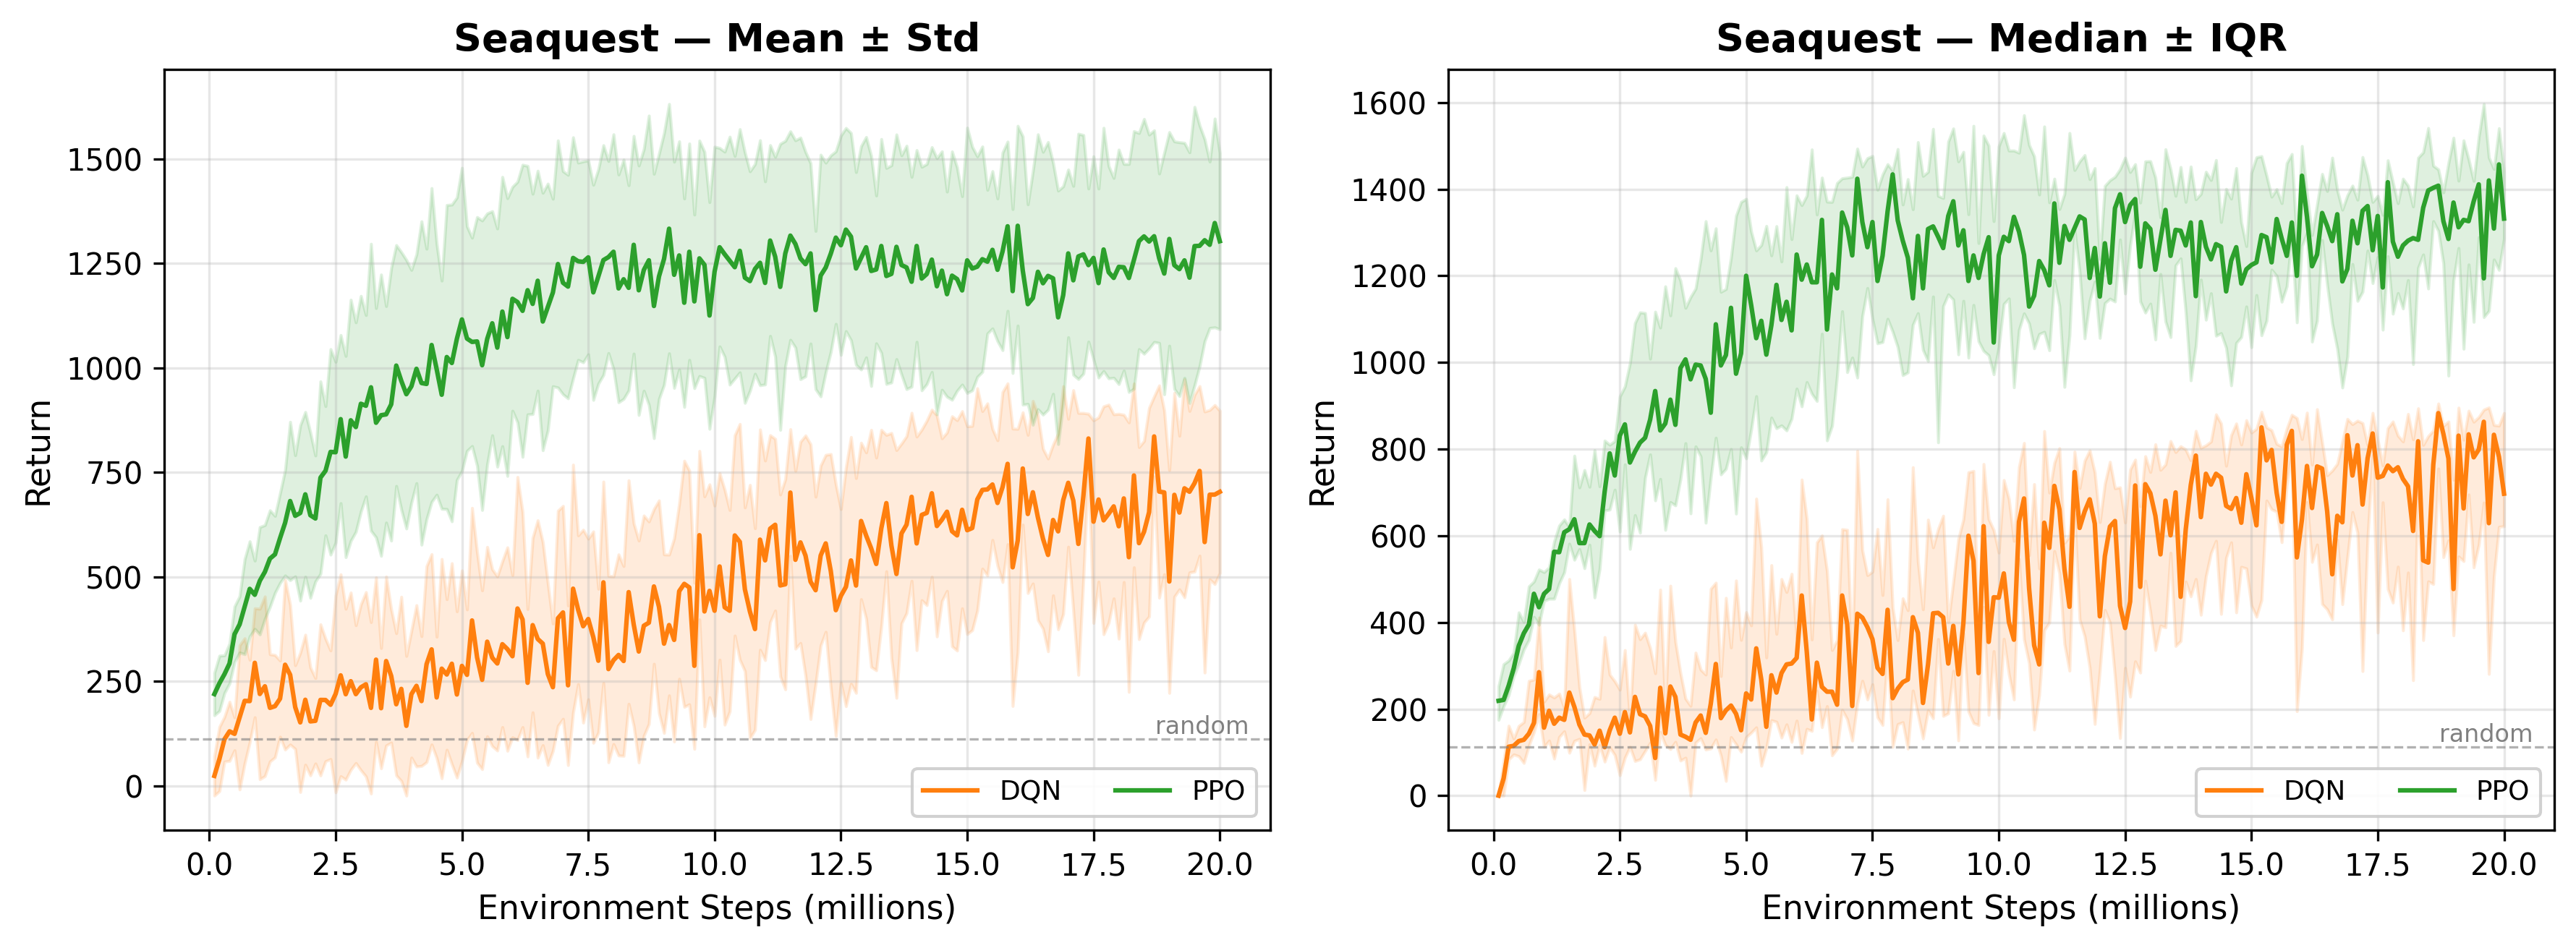
\includegraphics[width=0.8\textwidth]{learning_curves_seaquest.png}
  \caption{Learning curves on Seaquest, 10 seeds per algorithm, 20M steps.
  Note the multi-scale $y$-axis: raw returns span roughly two orders of
  magnitude.}
  \label{fig:exp3-lc-seaquest}
\end{figure}

\subsection*{6.6. Combined learning curves}

Normalised learning curves pooled across the three environments
(Fig.~\ref{fig:exp3-lc-combined}). The aggregate view is dominated by
whichever environment has the highest normalised ceiling, which is why
per-environment curves above are the primary evidence.

\begin{figure}[h]
  \centering
  
\includegraphics[width=0.85\textwidth]{combined_learning_curves.png}
  \caption{Combined normalised learning curves across Pong, Breakout,
  and Seaquest, 10 seeds per algorithm.}
  \label{fig:exp3-lc-combined}
\end{figure}

\subsection*{6.7. Score distributions and per-seed analysis}

\begin{figure}[h]
  \centering
  
\includegraphics[width=0.8\textwidth]{score_distribution.png}
  \caption{Distribution of normalised final scores per environment.
  DQN is concentrated in the mid-range on all three environments; PPO
  is bimodal, with Pong and Seaquest near their ceilings and Breakout
  near the floor.}
  \label{fig:exp3-score-dist}
\end{figure}

\begin{figure}[h]
  \centering
  
\includegraphics[width=0.8\textwidth]{per_seed_heatmap.png}
  \caption{Heatmap of normalised final scores by seed (rows) and
  environment (columns).}
  \label{fig:exp3-heatmap}
\end{figure}

\begin{figure}[h]
  \centering
  
\includegraphics[width=0.8\textwidth]{per_seed_boxswarm.png}
  \caption{Box-and-swarm plot of per-seed normalised scores.}
  \label{fig:exp3-boxswarm}
\end{figure}

\subsection*{6.8. Cross-environment aggregate results}

\begin{figure}[h]
  \centering
  
\includegraphics[width=0.75\textwidth]{final_performance.png}
  \caption{Cross-environment IQM, mean, and median with 95\% stratified
  bootstrap confidence intervals. DQN IQM 0.443 (CI [0.369, 0.521]),
  PPO IQM 0.277 (CI [0.247, 0.309]).}
  \label{fig:exp3-final-perf}
\end{figure}

\begin{figure}[h]
  \centering
  
\includegraphics[width=0.7\textwidth]{performance_profile.png}
  \caption{Performance profiles with 95\% bootstrap CIs.}
  \label{fig:exp3-perf-profile}
\end{figure}

\begin{figure}[h]
  \centering
  
\includegraphics[width=0.55\textwidth]{optimality_gap.png}
  \caption{Optimality gap. Lower is better. DQN 0.550 (CI [0.500, 0.607]),
  PPO 0.614 (CI [0.597, 0.632]).}
  \label{fig:exp3-opt-gap}
\end{figure}

\begin{figure}[h]
  \centering
  
\includegraphics[width=0.55\textwidth]{poi_heatmap.png}
  \caption{Pairwise probability of improvement: $P(\text{DQN}>\text{PPO})
  = 0.393$. Read as ``the chance that a randomly chosen DQN run scores
  higher than a randomly chosen PPO run''.}
  \label{fig:exp3-poi}
\end{figure}

\paragraph{The aggregation contradiction.}
The cross-environment IQM says DQN wins decisively (0.443 vs 0.277,
non-overlapping CIs). The pairwise probability of improvement says the
opposite: $P(\text{DQN}>\text{PPO}) = 0.393$, meaning a random PPO run
is more likely to beat a random DQN run than vice versa. Both numbers
are computed from the same 30-run score matrix.

The contradiction is not an error. IQM is robust to outliers by
trimming the top and bottom 25\% of the pooled $N \cdot M$ score values;
pairwise POI is computed \emph{per seed per environment} without
trimming and then averaged. Breakout is responsible for the flip: DQN's
Breakout dominance (roughly 4$\times$ PPO's score) lifts DQN's IQM
through its upper tail, while PPO's weaker-but-consistent per-seed
performance on Pong and Seaquest (both above DQN's median on those
environments) lets PPO win the majority of pairwise comparisons.

The practical lesson is that with $M=3$ environments and 10 seeds, the
choice of cross-env aggregation method can flip the conclusion. I report
\emph{both} aggregates rather than choosing one, and treat the
per-environment results (\S6.5) as the primary evidence.

\subsection*{6.9. Sample efficiency}

\begin{figure}[h]
  \centering
  
\includegraphics[width=0.85\textwidth]{sample_efficiency_pong.png}
  \caption{Sample efficiency on Pong (normalised AUC, 20M-step budget).}
  \label{fig:exp3-se-pong}
\end{figure}

\begin{figure}[h]
  \centering
  
\includegraphics[width=0.85\textwidth]{sample_efficiency_breakout.png}
  \caption{Sample efficiency on Breakout (normalised AUC, 20M-step budget).}
  \label{fig:exp3-se-breakout}
\end{figure}

\begin{figure}[h]
  \centering
  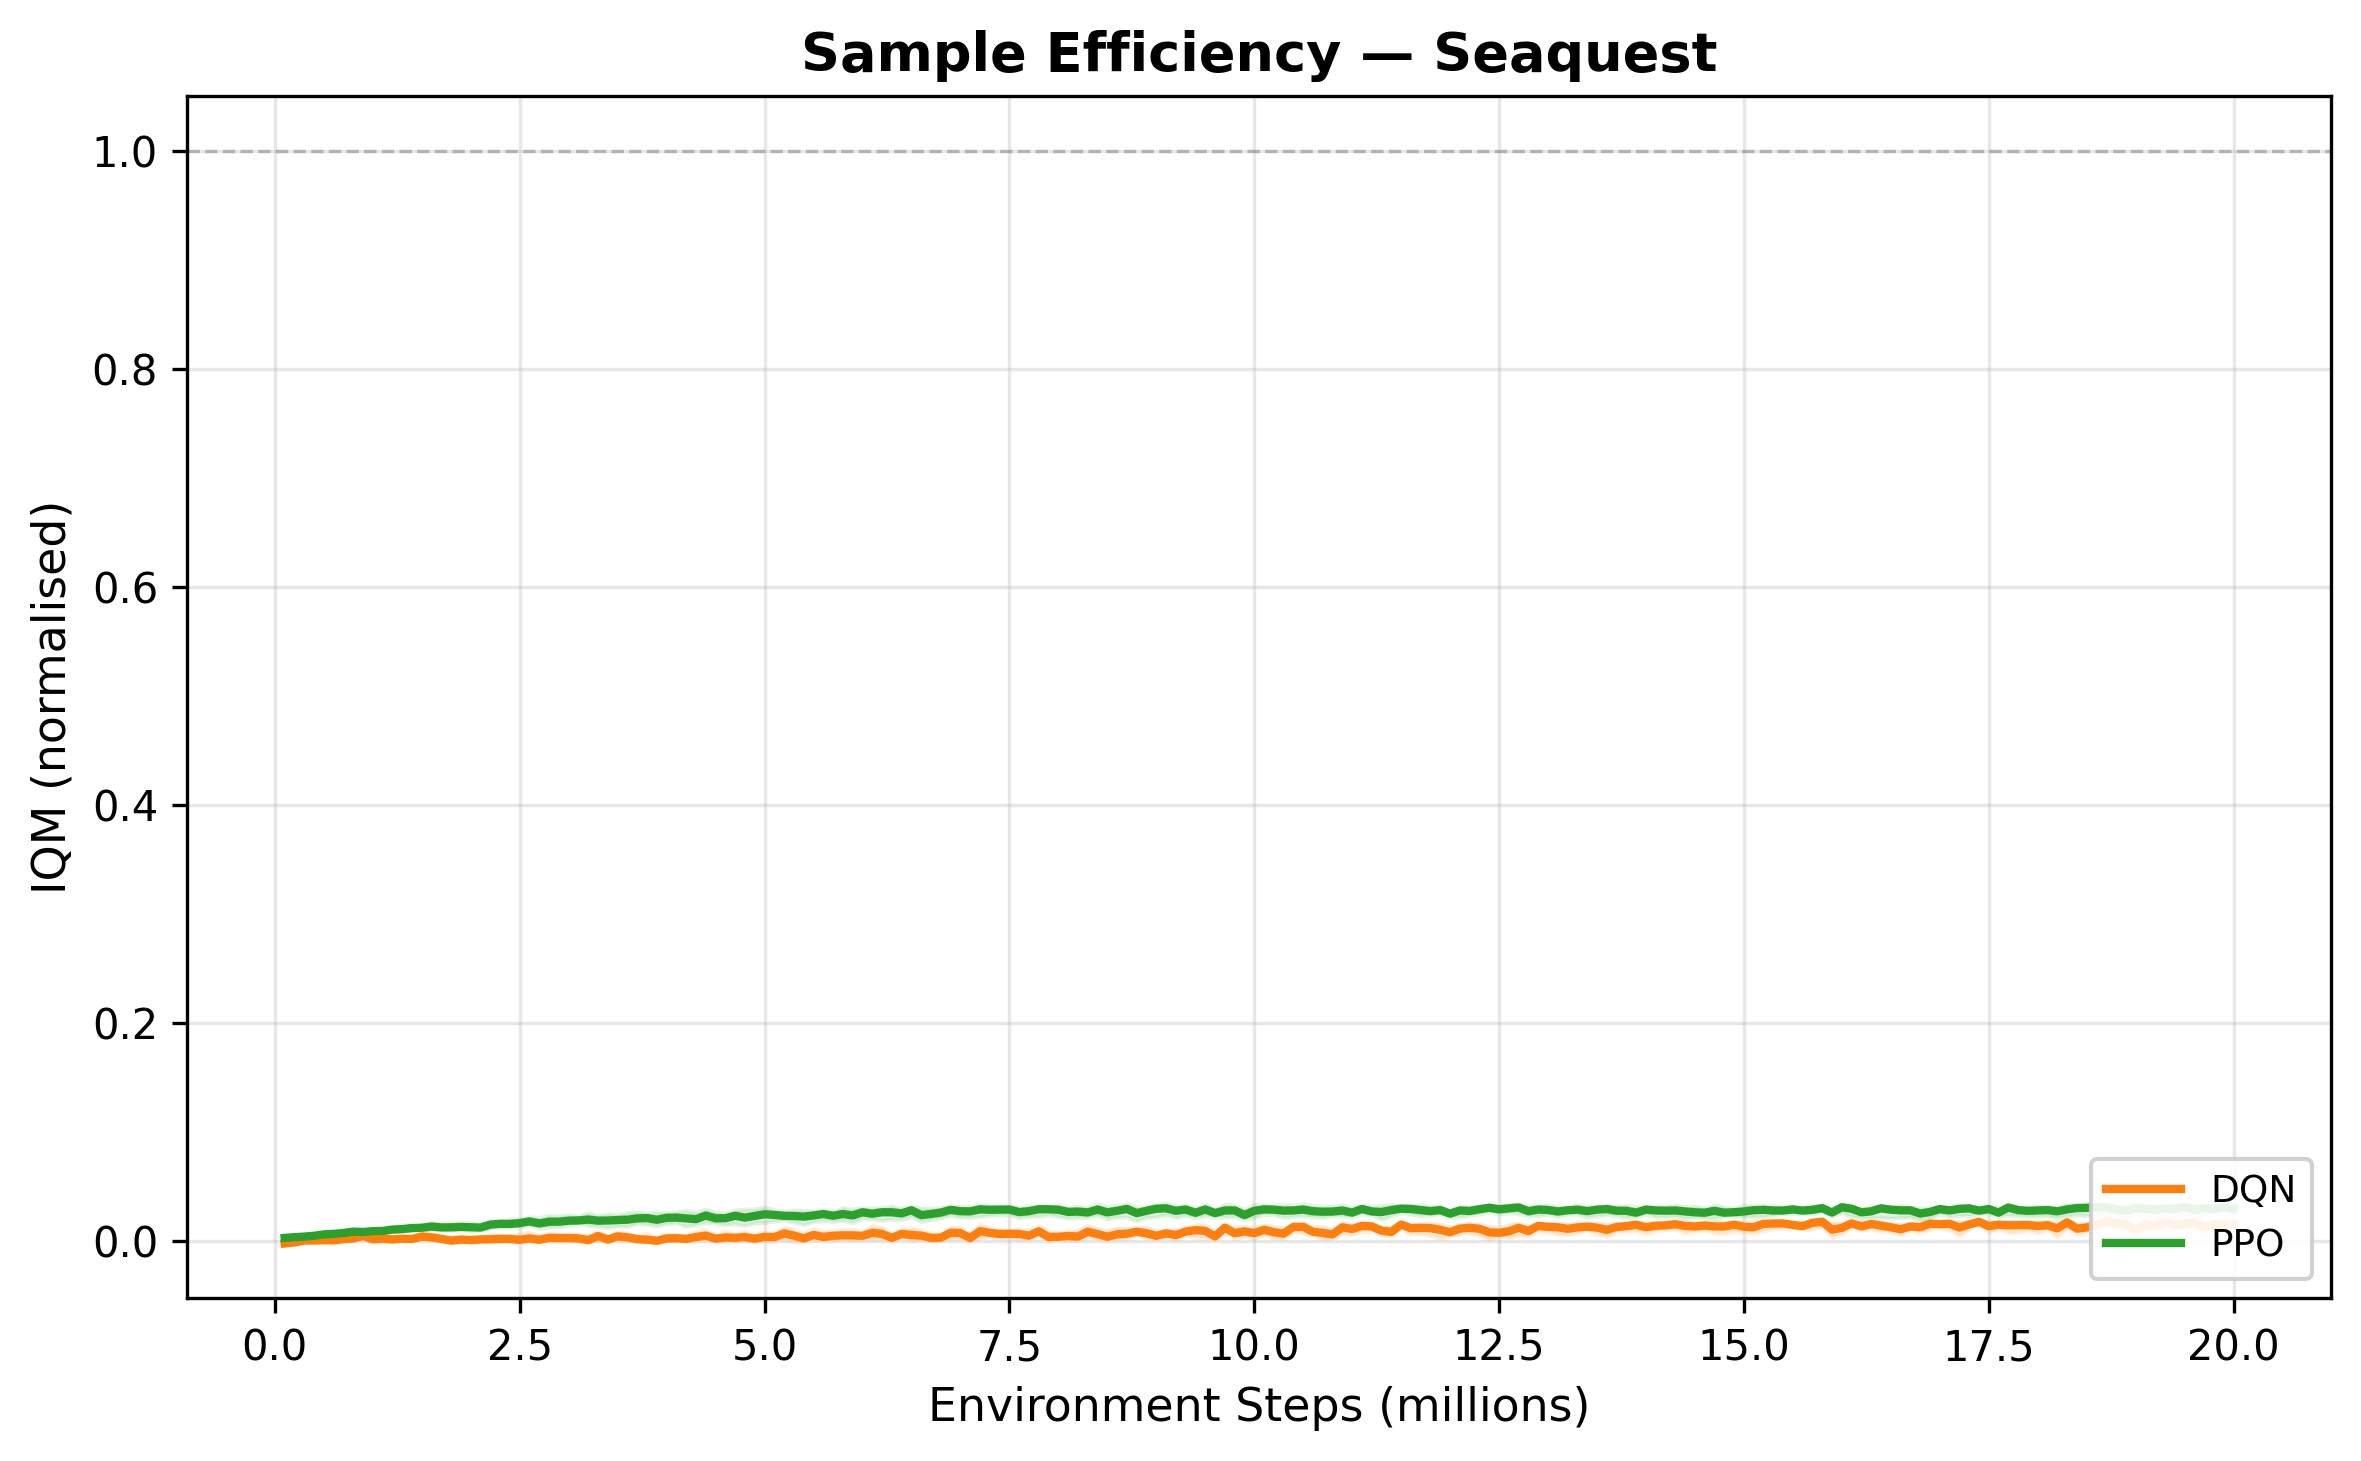
\includegraphics[width=0.85\textwidth]{sample_efficiency_seaquest.png}
  \caption{Sample efficiency on Seaquest (normalised AUC, 20M-step budget).}
  \label{fig:exp3-se-seaquest}
\end{figure}

\subsection*{6.10. Reproducibility finding}

Beyond the algorithm comparison, Experiment~3 yielded an unexpected and
useful secondary result: the training pipeline is \emph{bitwise
deterministic} on the target hardware. Retrained seeds
(\fileline{results\_of\_lost/} versus the original \fileline{results/})
produce identical final evaluation scores and identical
checkpoint-by-checkpoint learning curves when run on the same RTX~4090
with the same
\fileline{seed\_everything()} setup, the same driver version, and
\texttt{torch.use\_deterministic\_algorithms(True)}. This is unusual for
GPU-based RL --- the default assumption in the literature
\cite{henderson2018matters,patterson2024edrl} is that GPU non-determinism
makes exact bitwise reproduction infeasible.

\begin{figure}[h]
  \centering
  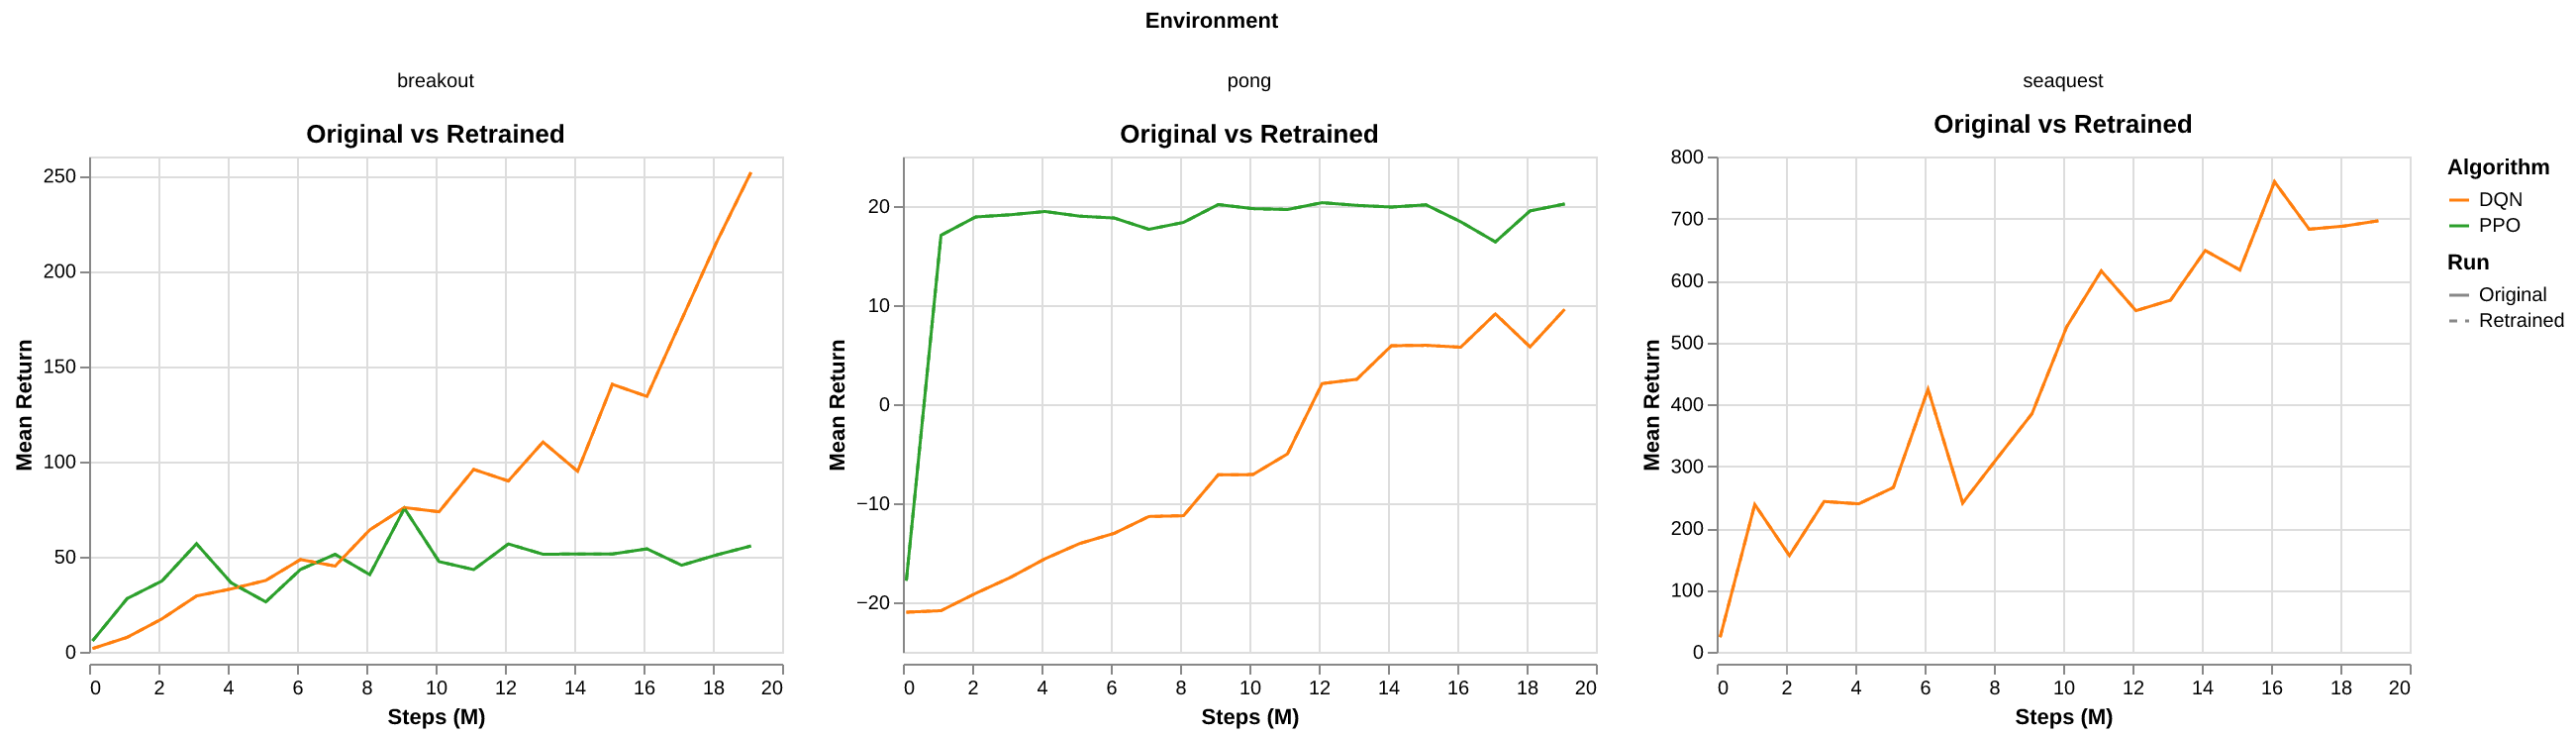
\includegraphics[width=0.85\textwidth]{reproducibility_learning_curves.png}
  \caption{Original vs retrained learning curves. Within floating-point
  noise the two runs of each seed are indistinguishable.}
  \label{fig:exp3-repro-lc}
\end{figure}

\begin{figure}[h]
  \centering
  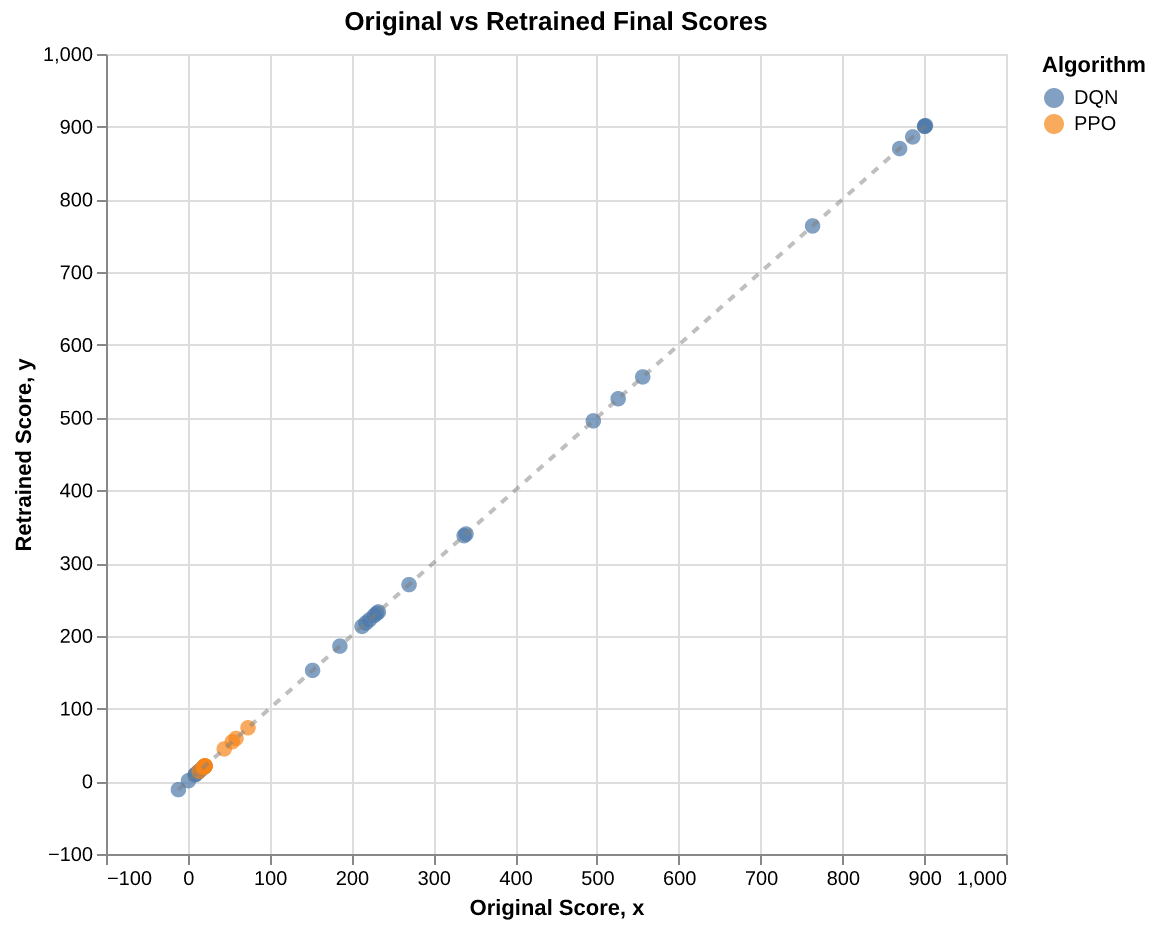
\includegraphics[width=0.65\textwidth]{reproducibility_scatter.png}
  \caption{Original vs retrained final scores. Perfect diagonal agreement
  ($r^2 \approx 1.0$, residuals at the floating-point noise floor).}
  \label{fig:exp3-repro-scatter}
\end{figure}

I note this as a practical finding rather than a theoretical claim:
future students attempting to reproduce this thesis on an RTX~4090 with
the pinned PyTorch and CUDA versions should expect exact numerical
agreement with the reported results.

\subsection*{6.11. Timing analysis}

\begin{figure}[h]
  \centering
  
\includegraphics[width=0.85\textwidth]{timing_per_seed.png}
  \caption{Per-seed wall-clock training time for the retrained runs
  (DQN only --- PPO timing is partially incomplete; see \S6.x
  Limitations).}
  \label{fig:exp3-timing}
\end{figure}

Retrained DQN wall-clock totals (10 seeds each, RTX~4090): 27.7 hours
for Pong, 17.4 hours for Breakout, 27.4 hours for Seaquest. Seaquest's
longer episodes and larger observation variance explain why it costs
slightly more wall-clock per run than Pong despite the identical
20M-step budget.

\subsection*{6.12. Key findings vs hypotheses}

\begin{itemize}[leftmargin=*]
  \item \textbf{H3.1 (PPO wins Pong) --- confirmed.} PPO mean 19.78 vs
  DQN 11.20.
  \item \textbf{H3.2 (DQN wins Breakout) --- confirmed, larger than
  expected.} DQN 229 vs PPO 65, a 3.5$\times$ margin.
  \item \textbf{H3.3 (both make progress on Seaquest) --- confirmed.}
  DQN 714, PPO 1174. Both clearly above the random baseline
  ($\approx 68$).
  \item \textbf{H3.4 (Exp~2 PPO aggregate survives) --- \emph{partially
  refuted}.} The IQM aggregate now favours DQN; the pairwise POI still
  favours PPO. This is the chapter's central finding.
  \item \textbf{H3.5 (aggregates remain fragile at $M=3$) ---
  confirmed.} The IQM / POI disagreement is itself evidence that $M=3$
  is still too small for aggregates to be robust to the choice of
  summary statistic.
\end{itemize}

\subsection*{6.13. Discussion}

\paragraph{Why does the aggregate flip?}
In Experiment~2 (Pong + Breakout, 5M steps), PPO's Pong dominance was
large enough to carry the cross-env aggregate despite DQN's Breakout
advantage. In Experiment~3 (Pong + Breakout + Seaquest, 20M steps), two
things change. First, DQN's Breakout lead grows: with 4$\times$ more
training steps, DQN's value iteration gets to exploit more of
Breakout's state space, pushing the DQN/PPO Breakout ratio from
\textasciitilde 1.3 to 3.5. Second, adding Seaquest adds a third
environment where the gap between algorithms is moderate rather than
extreme. The net effect is that DQN's Breakout tail becomes visible in
the IQM while PPO's advantage on Pong and Seaquest becomes ``merely''
1.6$\times$ rather than order-of-magnitude.

\paragraph{Per-environment is the primary evidence.}
The agreement between the IQM and POI aggregates in Experiments~1 and 2
made it easy to quote a single cross-env number. Experiment~3 is a
reminder that this agreement was incidental. When the two aggregates
disagree, per-environment performance is what matters and any ``which
algorithm is better'' framing has to be narrowed to ``better at what''.

\paragraph{Buffer size oversight.}
The DQN runs used \texttt{buffer\_size=100{,}000}
with \texttt{optimize\_memory\_usage=True}. The intended configuration
was a 400K buffer (closer to the original Nature paper). The smaller
buffer was used as an oversight during training-script configuration.
All DQN numbers reported here are with the 100K buffer. A follow-up
study with the intended 400K buffer would quantify how much of DQN's
Breakout lead is buffer-size sensitive; I expect the qualitative
finding (DQN wins Breakout, PPO wins Pong and Seaquest) to survive.

\subsection*{6.14. Limitations}

\begin{itemize}[leftmargin=*]
  \item \textbf{Default hyperparameters.} As in Experiments~1 and 2,
  no per-algorithm or per-environment tuning. The comparison is
  between ``out-of-the-box SB3 DQN'' and ``out-of-the-box SB3 PPO'' at
  the 20M-step budget.
  \item \textbf{Seed count.} 10 seeds per cell, matching
  Experiment~2 but fewer than Experiment~1's 15. Bootstrap CIs are
  correspondingly wider.
  \item \textbf{$M=3$ environments.} Still small. The IQM/POI
  disagreement above is direct evidence that $M=3$ is not enough for
  cross-env aggregates to be robust to the choice of summary
  statistic.
  \item \textbf{DQN buffer size.} 100K instead of the intended 400K
  (oversight).
  \item \textbf{Training timing incomplete.} The original Experiment~3
  training run lost its per-seed wall-clock logs due to an
  instrumentation issue. Retrained runs recovered full timing for DQN
  on all three environments but only a subset of PPO seeds. Evaluation
  scores are complete for all 30 runs; only fine-grained wall-clock
  comparisons are affected.
\end{itemize}

%=====================================================================
\section{Draft: Chapter 6 (Conclusions) expansion}\label{sec:conclusions}
%=====================================================================

\textbf{Scope note.} Draft for Nick to paste into
\fileline{6\_conclusions/conclusions.tex} (or
\fileline{7\_conclusions/conclusions.tex} after Experiment~3 is
promoted). Tone: restate, synthesise, answer, acknowledge, forward.

\subsection*{Draft content}

\paragraph{Restated research question.}
``How does the performance of value-based Deep Q-Network agents compare
to actor-critic agents (specifically PPO and A2C) in discrete-action
environments, including their sample efficiency and training
consistency?''

\paragraph{Synthesis of Experiment 1 (classic control, $M=3$, 15 seeds).}
On CartPole-v1, Acrobot-v1, and LunarLander-v3, PPO and A2C decisively
outperform the DQN family. PPO achieves a normalised IQM of 0.981 across
the three environments, with probabilities of improvement over every
other algorithm of at least 0.89. The DQN family (DQN and QR-DQN) fails
to learn at the allowed training budget (200K steps for CartPole and
Acrobot, 500K for LunarLander), scoring at or near random. RPPO
collapses on Acrobot in a way that indicates its recurrent policy is
ill-suited to fully-observable MDPs. Classic-control is not a DQN
environment at this budget.

\paragraph{Synthesis of Experiment 2 (Atari 5M, $M=2$, 10 seeds).}
Moving to Atari with CNN policies at 5M environment steps per seed flips
the per-environment ranking partially. On Pong, PPO continues to
dominate (mean return $\approx 20$ vs DQN $\approx -8$). On Breakout,
DQN slightly outperforms PPO, though both remain well below 11\% of the
theoretical maximum. The cross-environment aggregate still favours PPO
($\text{IQM}_{\text{PPO}}=0.529$ vs $\text{IQM}_{\text{DQN}}=0.130$,
$P(\text{PPO}>\text{DQN})=0.648$), but the margin is much smaller than
in classic control, and the $M=2$ aggregate is visibly dominated by
Pong's dynamic range.

\paragraph{Synthesis of Experiment 3 (Atari 20M, $M=3$, 10 seeds).}
Extending the budget to 20M steps and adding Seaquest as a third Atari
environment produces the chapter's most interesting result: the
cross-environment aggregate \emph{flips}. The IQM now favours DQN
($0.443$ vs $0.277$), driven by DQN's 3.5$\times$ Breakout lead at the
larger budget. The pairwise probability of improvement, however, still
favours PPO ($P(\text{DQN}>\text{PPO})=0.393$). Per-environment, DQN
wins Breakout decisively, PPO wins Pong and Seaquest moderately. The
practical takeaway is that the IQM/POI disagreement is itself a finding:
with $M=3$ environments and 10 seeds, the choice of cross-environment
aggregation method can flip the answer to ``which algorithm is better''.
Secondarily, Experiment~3 established that the training pipeline is
bitwise deterministic on the target RTX~4090 hardware --- a practical
result for anyone attempting to reproduce this work.

\paragraph{Answer to the research question.}
Neither family dominates. The correct comparison is per-environment, and
even within Atari the ranking depends on the environment, the budget,
and the aggregation method:
\begin{itemize}[leftmargin=*]
  \item On dense-reward, low-dimensional, fully-observable classic
  control, PPO and A2C are clearly stronger than DQN and QR-DQN at the
  budgets tested.
  \item On Atari Pong, PPO is consistently stronger at both 5M and 20M
  step budgets.
  \item On Atari Breakout, DQN edges PPO at 5M and wins decisively at
  20M.
  \item On Atari Seaquest at 20M, PPO wins moderately.
  \item Cross-environment aggregates are fragile at the $M$ values used
  here, and the choice of IQM vs pairwise POI can flip the aggregate
  answer. Per-environment reporting is the primary evidence.
\end{itemize}

\paragraph{Limitations.}
\begin{itemize}[leftmargin=*]
  \item \textbf{Default hyperparameters across the board.} No per-algorithm
  tuning. This keeps the comparison fair but means the numbers are
  ``out-of-the-box SB3'' rather than ``best achievable''.
  \item \textbf{Small $M$.} Classic control uses $M=3$, Atari uses $M=2$
  (Exp~2) then $M=3$ (Exp~3). All below the $M=$ 50+ used in standard RL
  benchmark papers.
  \item \textbf{Fixed training budgets.} 200K--500K on classic control,
  5M on Atari-Exp-2, 20M on Atari-Exp-3. These are smaller than the
  original DQN/PPO paper budgets (50M frames) and almost certainly
  disadvantage DQN more than PPO.
  \item \textbf{Experiment~3 buffer size oversight.} 100K instead of the
  intended 400K.
  \item \textbf{PPO timing data incomplete for Experiment~3.} Evaluation
  scores are complete; only per-seed wall-clock timing has gaps.
\end{itemize}

\paragraph{Future work.}
\begin{itemize}[leftmargin=*]
  \item Repeat Experiment~3 with the intended 400K DQN buffer size.
  \item Longer budgets (50M+ frames on Atari) to catch up with the
  original DQN and PPO paper settings.
  \item Larger $M$: add more Atari environments (SpaceInvaders, MsPacman,
  BeamRider) and more classic-control environments (MountainCar,
  Pendulum) so cross-env aggregates are less fragile.
  \item Hyperparameter tuning study on one environment per algorithm to
  quantify the gap between ``default SB3'' and ``best tuned''.
  \item MuJoCo or continuous-control study to see whether the
  per-environment pattern seen here generalises beyond discrete-action
  domains.
\end{itemize}

%=====================================================================
\section{Draft: scrubbed DQN$\times$Pong timing text}\label{sec:scrub}
%=====================================================================

Two tones. Nick picks one, per Q-F.

\subsection*{Tone (a): omit entirely}

\textbf{Replacing \fileline{5\_chapter/chapter.tex:68--75}:} simply
delete the paragraph and the red TODO. No substitute text. The existing
sentence immediately before it continues naturally to the Training
Summary subsection.

\textbf{Replacing \fileline{5\_chapter/chapter.tex:184--194}:} replace
the entire paragraph with:

\begin{quote}
\textit{DQN$\times$Pong wall-clock training time was comparable to
PPO$\times$Pong at the per-seed level (see the timing figure above).
Fine-grained wall-clock comparisons across seeds are not reported due
to incomplete per-seed timing instrumentation.}
\end{quote}

\textbf{Replacing \fileline{5\_chapter/chapter.tex:553--557}:} delete
the entire paragraph (the caveat). No substitute.

\subsection*{Tone (b): one-line disclosure}

\textbf{Replacing \fileline{5\_chapter/chapter.tex:68--75}:}

\begin{quote}
\textit{A methodological note: consistent per-seed wall-clock training
time could not be captured for all runs due to an instrumentation issue
during training. Evaluation scores are complete for all seeds and are
the primary evidence reported in this chapter; wall-clock timing
comparisons should be interpreted with care.}
\end{quote}

\textbf{Replacing \fileline{5\_chapter/chapter.tex:184--194}:}

\begin{quote}
\textit{Aggregate DQN and PPO wall-clock timings on Pong are similar
(\ldots\ hours each for 10 seeds). Finer-grained per-seed comparisons
are not reported because the training instrumentation did not capture
per-seed timing uniformly across runs.}
\end{quote}

\textbf{Replacing \fileline{5\_chapter/chapter.tex:553--557}:} delete the
entire caveat paragraph; tone-(b) disclosure at the top of the chapter
already covers it.

%=====================================================================
\section{Draft: chapter-top summary paragraphs}\label{sec:summaries}
%=====================================================================

3--5 sentence opening paragraphs for each chapter. Paste under the
\fileline{\textbackslash chapter\{...\}} line.

\subsection*{Chapter 4 (Classic-Control Benchmark)}

\begin{quote}
\textit{This chapter reports Experiment~1: a classic-control benchmark
comparing five algorithms (DQN, QR-DQN, A2C, PPO, RPPO) on three
environments (CartPole-v1, Acrobot-v1, LunarLander-v3) with 15 seeds
each and MlpPolicy on CPU. The primary evidence is per-environment; the
secondary aggregates summarise across the three tasks without claiming
general transfer. The headline result is that PPO and A2C dominate the
DQN family at the 200K--500K step budgets used here, with PPO achieving
a cross-environment IQM of 0.98. The chapter discusses the setup, the
per-environment results, the cross-environment aggregates, and the
failures (DQN family on CartPole, RPPO on Acrobot).}
\end{quote}

\subsection*{Chapter 5 (Atari Benchmark)}

\begin{quote}
\textit{This chapter reports Experiment~2: an Atari benchmark comparing
DQN and PPO on Pong and Breakout with 10 seeds per cell, CnnPolicy,
GPU training, and a 5M-step-per-seed budget. I focus on the two
``most representative'' algorithm families --- value-based (DQN) and
actor-critic (PPO) --- and use the same rliable-style metrics as
Chapter~4. The headline finding is that PPO wins Pong decisively while
DQN edges Breakout, and the cross-environment aggregate at $M=2$
environments is dominated by whichever per-environment gap is larger.
The chapter then discusses why $M=2$ aggregates are fragile, motivating
Experiment~3 (Chapter~6).}
\end{quote}

\subsection*{Chapter 6 (Experiment 3)}

\begin{quote}
\textit{This chapter reports Experiment~3: an extended Atari benchmark
that grows the training budget from 5M to 20M environment steps per
seed and adds Seaquest as a third environment, producing the thesis'
most interesting result. At the larger budget the cross-environment IQM
flips in favour of DQN (0.443 vs 0.277), driven by DQN's 3.5$\times$
Breakout advantage, but the pairwise probability of improvement still
favours PPO. This IQM/POI disagreement is itself a finding about the
fragility of cross-env aggregates at $M=3$. As a secondary result, the
training pipeline is shown to be bitwise deterministic on the target
RTX~4090 hardware, enabling exact reproduction of every reported number.}
\end{quote}

%=====================================================================
\section{Draft: PPO and A2C additions for the Literature Review}\label{sec:ppoa2c}
%=====================================================================

\textbf{Scope note.} These are drafts for Nick to insert into Chapter~2
after the generic Actor-Critic section at
\fileline{2\_literature\_review/literature\_review.tex:625}. Both
citations are already in \fileline{ref.bib}
(\fileline{mnih2016a3c}, \fileline{schulman2017ppo}).

\subsection*{Draft §2.x Advantage Actor-Critic (A2C)}

\begin{quote}
\textit{Advantage Actor-Critic (A2C) is a synchronous variant of
Mnih~et~al.'s Asynchronous Advantage Actor-Critic (A3C)
\cite{mnih2016a3c}. The core insight behind both methods is the use of
the advantage function
$A(s,a) = Q(s,a) - V(s)$
as the baseline-subtracted policy-gradient signal: instead of updating
the policy in proportion to the absolute return, the update is
proportional to how much better the taken action was than the critic's
state-value estimate. This reduces gradient variance substantially
without introducing bias, which is the same variance-reduction trick
that REINFORCE-with-baseline uses in a Monte-Carlo setting.}

\textit{A3C runs multiple actor threads in parallel, each carrying its
own environment and accumulating gradients asynchronously against a
shared parameter server. A2C, as implemented in
Stable-Baselines3~\cite{raffin2021sb3}, replaces the asynchronous update
with a synchronous one: $N$ parallel environments step together and
produce a batch of advantages that is used for a single combined
gradient update. The synchronous variant preserves the wall-clock
parallelism while simplifying reasoning about stale gradients, and it
has been shown to match A3C's performance when the batch size is
matched.}

\textit{A2C's relevant hyperparameters are the number of parallel
environments $n_{\text{envs}}$, the rollout length $n_{\text{steps}}$
(which together determine the batch size), the generalised-advantage
discount $\lambda_{\text{GAE}}$, the entropy regularisation
coefficient, and the value loss coefficient. In the experiments
reported in this thesis I use the Stable-Baselines3 default
hyperparameters without per-environment tuning.}
\end{quote}

\subsection*{Draft §2.x Proximal Policy Optimization (PPO)}

\begin{quote}
\textit{Proximal Policy Optimization \cite{schulman2017ppo} is the most
widely used actor-critic algorithm in deep reinforcement learning
today. Its design sits between two families: the high-variance,
single-step Monte-Carlo policy-gradient methods like REINFORCE and A2C,
and the more aggressive trust-region methods that maximise policy
improvement per update at the cost of complex constrained optimisation
(e.g.~TRPO). PPO targets the same ``take the biggest safe policy step''
goal as TRPO but replaces TRPO's constrained second-order update with a
first-order update against a clipped surrogate objective.}

\textit{The clipped surrogate objective is the heart of PPO. Let
$r_t(\theta) = \pi_\theta(a_t \mid s_t) \,/\, \pi_{\theta_{\text{old}}}(a_t
\mid s_t)$ denote the importance-sampling ratio between the new and old
policies at time $t$. PPO's policy loss is
$\mathbb{E}_t \big[\min\!\big(r_t(\theta)\,\hat A_t,\,
\mathrm{clip}(r_t(\theta),\,1-\epsilon,\,1+\epsilon)\,\hat A_t\big)\big]$,
where $\hat A_t$ is a generalised-advantage-estimate of the advantage.
The $\min$ of the raw and clipped objectives prevents the policy from
moving too far from $\pi_{\theta_{\text{old}}}$ in a single update: if
the unclipped update would push the ratio above $1+\epsilon$, the clip
blocks further improvement in that direction, and vice versa for
$1-\epsilon$.}

\textit{PPO combines this clipped policy loss with a value-function
loss and an entropy bonus, uses Generalised Advantage Estimation
\cite{schulman2015gae} for the advantages, and runs multiple epochs of
minibatch SGD over each rollout. Relative to A2C, the minibatch reuse
improves sample efficiency; relative to TRPO, the clipped objective
simplifies implementation enormously and has become the de facto
baseline algorithm in much of the deep RL literature.}

\textit{The relevant PPO hyperparameters are $n_{\text{envs}}$,
$n_{\text{steps}}$, the minibatch size, the number of epochs per
rollout (\texttt{n\_epochs}), the clip range $\epsilon$ (typically
0.1--0.2), $\lambda_{\text{GAE}}$, and the value / entropy loss
coefficients. As with A2C, I use the Stable-Baselines3 defaults
throughout this thesis and explicitly do not tune per-environment, to
keep the cross-algorithm comparison fair.}
\end{quote}

%=====================================================================
\section*{End of scratchpad}
%=====================================================================

Last revised 2026-04-11 as part of pre-submission planning. Nothing in
this document has been merged into the main thesis build. When Nick
is ready to action an item, he copies the relevant draft across and
ticks the corresponding checkbox in \S\ref{sec:todo}.

\end{document}
